\section{Phonon final states at small momentum}\label{sec:12.4}

A dark-matter particle of \SI{2}{MeV} can transfer a momentum of at most $q = 2\mchi v_{\mathrm{max}} = \SI{10.6}{keV}$. At $q = \SI{10}{keV}$ a silicon nucleus would recoil with $E_R = \SI{1.9}{meV}$, less than the energy of most phonons, and the Debye--Waller exponent is $2W_\kappa = 0.063$: in \SI{94}{\percent} of the kicks the lattice is left exactly as it was (\cref{sec:11.3}). Yet the particle carries enough kinetic energy, $\frac12\mchi v_{\mathrm{max}}^2 = \SI{7}{eV}$, to make an electron--hole pair. If the electrons do not follow the kicked nucleus, a pair is made while the lattice stays in its ground state, and the whole deposit is electronic. The free recoil of \cref{sec:12.3} is the wrong lattice factor here; the impulse regime of \cref{sec:11.4} begins only at \SI{92.5}{keV}, that is at $\mchi = \SI{17.5}{MeV}$. Below it the lattice factor of the Migdal entry is the multiphonon response of \cref{sec:11.3} (\cref{sec:12.1-counting}).

Does the leading entry \cref{eq:12.1-Skk}, derived with a nucleus that is free during the electronic time, hold for a bound nucleus, and with the momentum $p$ taken by the electrons as large as the kick itself? It does, to a few parts in $10^3$ (\cref{sec:12.4-amp}). The real question at small $q$ is how a Migdal event shares its energy between electrons and lattice when the lattice can take zero, one or a few phonons.

\subsection{The amplitude of a bound nucleus}\label{sec:12.4-amp}

Write the Migdal process as two perturbations acting in turn: the kick $\ee^{\ii\vect{q}\cdot\vect{X}_I}$ from the dark matter, and the potential of nucleus $I$ acting on the electrons. By \cref{app:D.33-amp}, that potential is a sum of Fourier components $v_\kappa(\vect{p})\,\ee^{-\ii\vect{p}\cdot\vect{X}_I}\,n_e(\vect{p})$, and the electronic factor $v_\kappa(\vect{p})\langle\Psi_j|n_e(\vect{p})|\Psi_0\rangle$ is common to every term below. What depends on the lattice is the nuclear factor. Let $H_N$ be the Hamiltonian of the nuclei on the ground surface, with eigenstates $|\lambda\rangle$ of energy $E_\lambda$, the initial one $|0\rangle$. The two orderings of \cref{eq:2.4-orderings} give, for a final lattice state $f$ and electronic energy $\omega_e$,
\begin{equation}
  \mathcal{A}_f(\vect{q},\vect{p}) = \sum_\lambda\left[\frac{\langle f|\ee^{-\ii\vect{p}\cdot\vect{X}_I}|\lambda\rangle\langle\lambda|\ee^{\ii\vect{q}\cdot\vect{X}_I}|0\rangle}{\omega_e + E_f - E_\lambda}
  - \frac{\langle f|\ee^{\ii\vect{q}\cdot\vect{X}_I}|\lambda\rangle\langle\lambda|\ee^{-\ii\vect{p}\cdot\vect{X}_I}|0\rangle}{\omega_e + E_\lambda - E_0}\right] .
  \label{eq:12.4-exact}
\end{equation}
In the first ordering the kick acts first and the nucleus then passes $\vect{p}$ to the electrons; the denominator is the energy of the final state minus that of the intermediate one. In the second the electrons are excited first, by the nucleus at rest, and the intermediate state carries $\omega_e$ in addition to the lattice energy. This is the amplitude of Berghaus and collaborators~\cite[Eq.~(3.1)]{berghaus2023migdal}, with their lattice states as the $|\lambda\rangle$.

The electronic energy is large against the lattice energies that the matrix elements allow, and the denominators can be expanded in powers of $1/\omega_e$. Call $A = \ee^{-\ii\vect{p}\cdot\vect{X}_I}$ and $B = \ee^{\ii\vect{q}\cdot\vect{X}_I}$. Since $\langle f|H_N = E_f\langle f|$ and $H_N|0\rangle = E_0|0\rangle$, each power of $(E_f - E_\lambda)$ in the first term turns into a commutator with $H_N$ acting on $A$ from the left, and each power of $(E_\lambda - E_0)$ in the second into the same commutator acting on $A$ from the right. Order by order,
\begin{equation}
  \mathcal{A}_f = \frac{\langle f|[A,B]|0\rangle}{\omega_e} + \frac{\langle f|[[A,H_N],B]|0\rangle}{\omega_e^2} + \frac{\langle f|[[[A,H_N],H_N],B]|0\rangle}{\omega_e^3} + \cdots .
  \label{eq:12.4-series}
\end{equation}
The first term vanishes, since $A$ and $B$ are functions of the same position. For the second, $H_N = \sum_I\vect{P}_I^2/2M_\kappa + U(\{\vect{X}\})$ with any interatomic potential $U$. The potential commutes with $A$; the kinetic energy does not, because $A$ shifts the momentum of nucleus $I$ by $-\vect{p}$, $A\vect{P}_IA^\dagger = \vect{P}_I + \vect{p}$. Hence
\begin{equation*}
  [A,H_N] = \Bigl(\frac{\vect{p}\cdot\vect{P}_I}{M_\kappa} + \frac{p^2}{2M_\kappa}\Bigr)A , \qquad
  [[A,H_N],B] = \frac{\vect{p}}{M_\kappa}\cdot[\vect{P}_I,B]\,A = \frac{\vect{q}\cdot\vect{p}}{M_\kappa}\,\ee^{\ii(\vect{q}-\vect{p})\cdot\vect{X}_I} ,
\end{equation*}
and the leading nuclear factor is
\begin{equation}
  \mathcal{A}^{(2)}_f = \frac{\vect{q}\cdot\vect{p}}{M_\kappa\,\omega_e^2}\,\bigl\langle f\big|\ee^{\ii(\vect{q}-\vect{p})\cdot\vect{X}_I}\big|0\bigr\rangle .
  \label{eq:12.4-lead}
\end{equation}
This is the nuclear factor of \cref{eq:12.1-amp}, now obtained without any assumption about the binding of the nucleus. The interatomic potential has dropped out, as Berghaus and collaborators showed with their effective Hamiltonian $\nabla_IH_{\chi L}\cdot\nabla_IH_{eL}/(m_N\omega^2)$~\cite[Eq.~(3.6)]{berghaus2023migdal}. Esposito and Rocchi obtained the same matrix element from the first nonadiabatic correction to the Born--Oppenheimer product state~\cite[Eq.~(21)]{esposito2025migdal}, and showed that in an infinite crystal, whose center of mass does not move, the adiabatic part of the amplitude vanishes. Two routes therefore give one result: the boost of \cref{sec:8.6} and the second-order amplitude with the lattice integrated out.

The lattice enters at the next order, and the expansion shows what controls it. With $X = \vect{p}\cdot\vect{P}_I/M_\kappa + p^2/2M_\kappa$, the same steps give $[[[A,H_N],H_N],B] = (\vect{q}\cdot\vect{p}/M_\kappa)(2X - \vect{q}\cdot\vect{p}/M_\kappa)\,BA$, plus a term $-\ii(\vect{p}\cdot\nabla_IU/M_\kappa)A$ that commutes with $B$ and drops out. The potential first appears at order $\omega_e^{-4}$, through $[\vect{p}\cdot\nabla_IU,\vect{P}_I]$, the force constants. Summing $|\mathcal{A}_f|^2$ over all final states, averaging over the direction of $\vect{p}$ with the weight $(\vect{q}\cdot\vect{p})^2$ of the leading term, and collecting the terms of the first two orders,
\begin{equation}
  \frac{\sum_f|\mathcal{A}_f|^2}{\sum_f|\mathcal{A}^{(2)}_f|^2} = 1 - \frac{2p^2}{M_\kappa\,\omega_e} + \frac{2\langle\omega_{\mathrm{ph}}^2\rangle}{\omega_e^2} + \frac95\,\frac{v_N^2p^2}{\omega_e^2} + \cdots ,
  \label{eq:12.4-corr}
\end{equation}
with $v_N = q/M_\kappa$ and $\langle\omega_{\mathrm{ph}}^2\rangle$ the mean square phonon frequency seen by the nucleus. The first correction is the recoil energy of the momentum given to the electrons, $p^2/2M_\kappa$, over $\omega_e$: the expectation value of $2X - \vect{q}\cdot\vect{p}/M_\kappa$ in the kicked state is $\vect{p}\cdot(\vect{q} - \vect{p})/M_\kappa$, whose part odd in $\vect{p}$ averages away. The second is the binding of the nucleus, the factor $[1 - (\omega_{\mathrm{ph}}/\omega_e)^2]^{-2}$ that \cref{sec:6.1} found for a nucleus kicked in a harmonic well, at its first order. The third is the Doppler shift of the electronic energy by the moving nucleus, $\vect{v}_N\cdot\vect{p}$, at second order: for a free nucleus, \cref{eq:12.4-exact} is the bracket \cref{eq:12.3-bracket} with $b = \vect{q}\cdot\vect{p}/M_\kappa$, whose expansion $(b/\omega_e^2)(1 + b/\omega_e + b^2/\omega_e^2 + \cdots)$ squared and averaged with $\langle c^4\rangle/\langle c^2\rangle = 3/5$ gives the coefficient $9/5$.

None of the three is a ratio $p/q$, so the leading factor \cref{eq:12.4-lead} holds when the electrons take as much momentum as the nucleus receives, or more, as for the free nucleus of \cref{eq:12.3-bracket}. For silicon at $p = \SI{5.7}{keV}$, the median momentum of the Migdal weight (\cref{sec:12.3}), and $\omega_e = \SI{1.2}{eV}$, near the gap, the three terms of \cref{eq:12.4-corr} are $-2.1\times10^{-3}$, $+2.8\times10^{-3}$ (with the silicon phonon spectrum) and at most $5.1\times10^{-4}$ for every $q$ up to the impulse onset. The leading factor is exact to a few parts in $10^3$ throughout the region of this section. \Cref{lim:12.4a} below compares it with the full sum.

\subsection{Migdal rate with phonon final states}\label{sec:12.4-rate}

Squaring \cref{eq:12.4-lead}, summing over the nuclei and keeping the diagonal $\vect{G} = \vect{G}'$ of the electronic response and the self part of the lattice factor gives the Migdal entry with the lattice factor of one nucleus at the momentum $\vect{q} - \vect{p}$ that it keeps. For one nucleus per site the self response is $S^{\mathrm{ad}}_{\kappa;\vect{G}\vect{G}}(\vect{q} - \vect{k},\omega_l) = 2\pi\nd_\kappa\,s^{\mathrm{inc}}_\kappa(\vect{q} - \vect{k} - \vect{G},\omega_l)$, with $s^{\mathrm{inc}}_\kappa(\vect{Q},\omega)$ the spectrum of one nucleus normalized to $\int\dd\omega\,s^{\mathrm{inc}}_\kappa = 1$, zero-phonon line included. The self part is exact for the phonon-emitting terms, which are incoherent, and, averaged over the zone, for the zero-phonon term at $q \gtrsim 2q_{\mathrm{BZ}}$. Below the impulse onset that factor is the harmonic self response of \cref{eq:11.3-inc}, a zero-phonon line of weight $\ee^{-2W_\kappa}$ and the $n$-phonon spectra $P^\kappa_n$ with the Poisson weights \cref{eq:5.6-poisson}.
\begin{keyresult}[The Migdal probability with phonon final states]
At $n_B = 2$, for the valence electrons with the frozen-core vertex $v_\kappa = -Z_{\mathrm{ion}}(p)e^2/p^2$ of \cref{eq:12.3-Zion} and the diagonal loss function, a kick $\vect{q}$ of a nucleus of species $\kappa$ at a cubic site of a harmonic crystal at $T = 0$, with the incoherent lattice factor, leaves electronic energy $\omega_e$ and lattice energy $\omega_l$ with the probability density
\begin{equation}
  \begin{split}
  \frac{\dd^2P_{\mathrm{Mig}}}{\dd\omega_l\,\dd\omega_e} = 4\alpha\int\frac{\dd^3p}{(2\pi)^3}\;&Z_{\mathrm{ion}}(p)^2\,\frac{(\vect{v}_N\cdot\vect{p})^2}{\omega_e^4\,p^2}\,L(\vect{p},\omega_e)\,\ee^{-2W_\kappa(\vect{q}-\vect{p})} \\
  &\times\Biggl[\underbrace{\delta(\omega_l)}_{\text{zero-phonon, }\mathcal{P}_0} + \underbrace{\sum_{n\ge1}\frac{[2W_\kappa(\vect{q}-\vect{p})]^n}{n!}\,P^\kappa_n(\omega_l)}_{\text{phonon-emitting, }\mathcal{P}_+}\Biggr] .
  \end{split}
  \label{eq:12.4-harm}
\end{equation}
Integrated over $\omega_l$, the bracket times $\ee^{-2W_\kappa}$ gives one for every $\vect{p}$, and $\dd P_{\mathrm{Mig}}/\dd\omega_e$ is \cref{eq:12.3-soft} at every $q$ in this incoherent lattice form. The coherent zero-phonon process of the whole lattice has the same electronic spectrum, averaged over directions, for $q \gtrsim 2q_{\mathrm{BZ}}$. For $q \ll q_{\mathrm{BZ}}$ \cref{eq:8.3-boostward} fixes it at $(m_e/M_\kappa)^2(2q^2/e^2)L(\vect{q},\omega_e)/(2\pi\nd_\kappa)$, with $L$ the head of $-\varepsilon^{-1}$: in silicon $1/14.9$ of \cref{eq:12.3-soft}, with median $\omega_e = \SI{17.4}{eV}$ at the plasmon against \SI{4.5}{eV}. Between the two the coherent response is not computed (\cref{tab:12-nuisances}).
\end{keyresult}
\noindent This is the rate formula of Berghaus and collaborators~\cite[Eq.~(3.8)]{berghaus2023migdal}, with their partial structure factor in the incoherent harmonic form~\cite[Eqs.~(4.1), (4.5)]{berghaus2023migdal} and their effective charge $Z(k)$ as $Z_{\mathrm{ion}}$. Their full structure factor $S(\vect{q} - \vect{k}_e - \vect{K}, E)$ is the electron-following response of \cref{eq:12.1-Skk} at the momentum the nucleus keeps.

The sum rule in the key result, which Berghaus and collaborators pointed out, says that the electronic spectrum does not depend on the lattice dynamics. It needs no soft limit, since the lattice factor has unit weight at every $\vect{q} - \vect{p}$, and no impulse approximation. The lattice enters the rate only through energy conservation. In the double rate the lattice factor replaces the free recoil of \cref{eq:12.3-rate}. The weight $\dd E_R = q\,\dd q/M_\kappa$ is unchanged, and the minimum speed becomes $\vmin = (\omega_e + \omega_l)/q + q/2\mchi$, so that for a heavy mediator
\begin{equation}
  \frac{\dd^2\mathcal{R}}{\dd\omega_l\,\dd\omega_e} = \frac{\rho_\chi\,\sigma_N}{2\mchi\,\mu_{\chi N}^2M_\kappa}\int\dd q\;q\,\eta\Bigl(\frac{\omega_e + \omega_l}{q} + \frac{q}{2\mchi}\Bigr)\frac{\dd^2P_{\mathrm{Mig}}}{\dd\omega_l\,\dd\omega_e} .
  \label{eq:12.4-rate}
\end{equation}
Since $\omega_l$ is a few meV against an $\omega_e$ of a few eV, $\dd\mathcal{R}/\dd\omega_e$ hardly depends on how the lattice takes its share: replacing the free recoil by the bound response leaves the silicon rate unchanged (\cref{lim:12.3b}). What the lattice factor decides is the second axis of the joint response, the energy that a phonon sensor sees together with the charge. Berghaus, Essig and McDuffie extended \cref{eq:12.4-rate} to the nonrelativistic effective operators of the dark-matter--nucleon interaction~\cite{berghaus2026migdal}. Each operator multiplies the same electronic and lattice factors by its own nuclear response, and the lattice factor is again read at the momentum $\vect{q} - \vect{p}$ that the nucleus keeps.

\begin{limitbox}[Migdal effect with phonon final states][lim:12.4a]
$\dd^2P/\dd\omega_l\,\dd\omega_e = 4\alpha\int\dd^3p/(2\pi)^3\,Z_{\mathrm{ion}}(p)^2(\vect{v}_N\cdot\vect{p})^2L(\vect{p},\omega_e)\,s^{\mathrm{inc}}_\kappa(\vect{q} - \vect{p},\omega_l)/(\omega_e^4p^2)$, from the effective interaction $\nabla H_{\chi L}\cdot\nabla H_{eL}/(M_\kappa\omega_e^2)$~\cite[Eqs.~(3.6), (3.8)]{berghaus2023migdal}.
\par\smallskip
{\centering
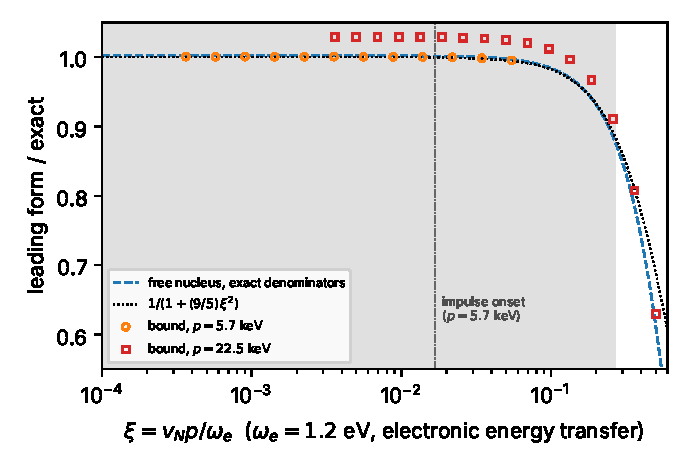
\includegraphics[width=\linewidth]{figures/ch12/limit12_4a.pdf}
\captionof{figure}{Migdal probability summed over all lattice final states, from the leading factor \cref{eq:12.4-lead}, divided by the same from the two time orderings \cref{eq:12.4-exact} with exact energy denominators, against $v_Np/\omega_e$ at the electronic energy transfer $\omega_e = \SI{1.2}{eV}$. Model: a silicon nucleus in an isotropic harmonic well of frequency $\omega_0 = \langle\omega^{-1}\rangle^{-1} = \SI{30.4}{meV}$, which has the Debye--Waller factor of the full phonon spectrum; direction of $\vect{p}$ averaged. Circles, $p = \SI{5.7}{keV}$ for $q = 2$ to \SI{300}{keV}; squares, $p = \SI{22.5}{keV}$ for $q$ up to \SI{700}{keV}, whose offset of 0.03 at small $v_Np/\omega_e$ is the recoil term $2p^2/M_\kappa\omega_e$. Dashed: free nucleus with exact denominators. Dotted: the leading correction $1/(1 + \frac95v_N^2p^2/\omega_e^2)$. Dash-dotted: the impulse onset at $p = \SI{5.7}{keV}$. Gray: within \SI{10}{\percent}, $v_Np/\omega_e \le 0.27$.}\label{fig:12-limit-4a}
\par}
\smallskip
The form fails when the Doppler shift $\vect{v}_N\cdot\vect{p}$ approaches $\omega_e$, at $q \approx \SI{1.5}{MeV}$ for $p = \SI{5.7}{keV}$ near the gap, far above the small-momentum region, where it holds to \num{e-3}.
\end{limitbox}

\noindent On the truncation label \cref{lim:12.4a} sits at $n_B = 2$, with $\mathfrak{M}$ = sudden, $\mathcal{K}$ = multiphonon at all orders (harmonic, incoherent), and $\mathcal{X}$ = random-phase with local fields on the diagonal. The diagonal is the approximation that costs most (\cref{sec:12.3-validity}).

\subsection{Zero-phonon, few-phonon and impulse regimes}\label{sec:12.4-regimes}

\Cref{fig:12-regimes} evaluates \cref{eq:12.4-harm} for silicon and sorts the Migdal events by the number of phonons they leave. The zero-phonon weight of the kick, $\ee^{-2W_\kappa(q)}$, falls to one half at $q = \SI{33.2}{keV}$, reached from $\mchi = \SI{6.3}{MeV}$. The impulse onset lies at \SI{92.5}{keV}. Below the first, most Migdal events are zero-phonon: at $q = \SI{10}{keV}$, \SI{92}{\percent} of them leave the lattice in its ground state, \SI{7.6}{\percent} emit one phonon and \SI{0.5}{\percent} two. Between the two boundaries a Migdal event emits a few phonons; at \SI{50}{keV} the fractions for zero, one, two and three or more are 0.21, 0.32, 0.25 and 0.22. Above the onset the lattice factor is the impulse Gaussian, and the soft-limit treatment of \cref{sec:12.3} holds.

\begin{figure}[tbp]
  \centering
  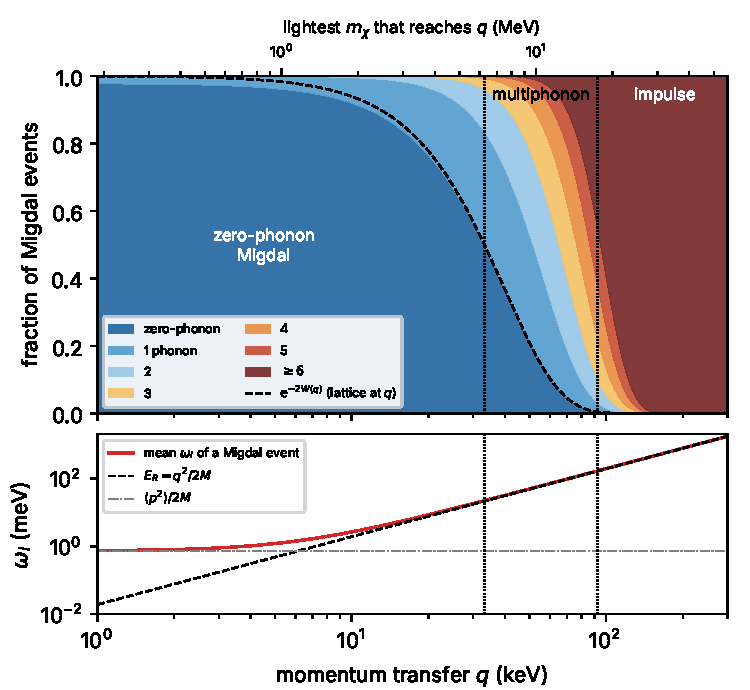
\includegraphics[width=0.84\linewidth]{figures/ch12/fig12_4.pdf}
  \caption{The three regimes of the Migdal effect in silicon against the momentum transfer $q$, at $T = 0$. Top: fraction of Migdal events that leave the lattice with zero, one, two, \ldots\ phonons, from \cref{eq:12.4-harm}, with the lattice factor at the momentum $\vect{q} - \vect{p}$ that the nucleus keeps, averaged over the momentum $\vect{p}$ given to the electrons with the weight $(\vect{q}\cdot\vect{p})^2Z_{\mathrm{ion}}(p)^2p^{-2}\int_{\Eg}\dd\omega_e\,L(p,\omega_e)/\omega_e^4$. Dashed: the zero-phonon weight $\ee^{-2W(q)}$ of the kick alone. Bottom: mean energy $\omega_l$ given to the lattice in a Migdal event, against the recoil energy $E_R$ and the recoil energy $\langle p^2\rangle/2M = \SI{0.72}{meV}$ of the electrons' momentum. Dotted lines: $\ee^{-2W(q)} = \frac12$ at \SI{33.2}{keV} and the impulse onset at \SI{92.5}{keV}. Top axis: the lightest dark matter that reaches $q$, $q/2v_{\mathrm{max}}$. Model: diagonal loss function with local fields of Knapen, Kozaczuk and Lin~\cite{knapen2021dark} (threshold \SI{1.11}{eV}, the step-model gap that accompanies the tables, $p \le \SI{22.5}{keV}$), $Z_{\mathrm{ion}}(p)$ of \cref{eq:12.3-Zion}, incoherent harmonic lattice factor with Poisson weights in $2W(Q) = Q^2\langle u_x^2\rangle$ from the PBE phonon spectrum of \cref{sec:5.2}.}
  \label{fig:12-regimes}
\end{figure}

At small $q$ the electrons' momentum controls the lattice. The momentum $p$ that the electrons take has $\langle p^2\rangle^{1/2} = \SI{6.1}{keV}$ in the weight of \cref{eq:12.4-harm}, and the nucleus keeps $\vect{q} - \vect{p}$, with $\langle|\vect{q} - \vect{p}|^2\rangle = q^2 + \langle p^2\rangle$. At \SI{5}{keV} this is 2.5 times $q^2$. The mean lattice energy of a Migdal event, $\langle|\vect{q} - \vect{p}|^2\rangle/2M_\kappa$ by the first moment of \cref{sec:11.3}, is then \SI{1.20}{meV}, 2.5 times the recoil energy, and at \SI{2}{keV} it is ten times $E_R$. The phonon-emitting fraction follows $2W_\kappa(\vect{q} - \vect{p})$, not $2W_\kappa(\vect{q})$: \SI{3.8}{\percent} at \SI{5}{keV}, against $1 - \ee^{-2W(q)} = \SI{1.6}{\percent}$. Above \SI{30}{keV} the difference fades, and at \SI{50}{keV} the mean lattice energy, \SI{48.5}{meV}, exceeds $E_R$ by \SI{1.5}{\percent}.

In the exact harmonic lattice factor, its part at $\omega_l = 0$ is the product of two ground-state expectation values of $n_\kappa$, which vanish unless $\vect{q} - \vect{p}$ is a reciprocal-lattice vector. A zero-phonon Migdal event is a Bragg process: the crystal takes a reciprocal-lattice vector $\vect{G}$ as a whole, with weight $\ee^{-2W_\kappa(\vect{G})}$ and the structure factor of the cell, and the electrons take exactly $\vect{p} = \vect{q} - \vect{G}$. The incoherent form in \cref{eq:12.4-harm} replaces this sum over discrete momenta by an integral over $\vect{p}$, which is its average over the zone (\cref{sec:11.3}). The two agree when the electronic weight varies slowly over $q_{\mathrm{BZ}}$. For silicon, averaging over the direction of $\vect{q}$ and keeping the diamond structure factor $|1 + \ee^{\ii\vect{G}\cdot\vect{\tau}}|^2$, the Bragg sum is 1.08, 1.04 and 1.03 times the incoherent integral at $q = 1.5$, 3 and \SI{5}{keV}, and within \SI{1}{\percent} of it from \SI{10}{keV}. This check keeps the diagonal $\vect{G} = \vect{G}'$ and averages over directions; the cross-site terms $\vect{G} \neq \vect{G}'$ of the coherent sum, which carry the screening of \cref{eq:8.3-boostward} at $q \ll q_{\mathrm{BZ}}$, are not tested by it. The electronic weight is spread over several zones, median $p = 2.5\,q_{\mathrm{BZ}}$, and the coherent sum samples it densely enough. For a fixed direction of $\vect{q}$ in a crystal at rest the sum depends on the orientation, which a direction-averaged rate does not see.

Germanium follows the same pattern at shifted boundaries. It has no first-principles phonon spectrum in this book (\cref{tab:5-phonons}). An estimate from its Debye temperature of \SI{373}{K}, scaled by the ratio 0.82 of the computed to the Debye value of $\langle\omega^{-1}\rangle^{-1}$ in silicon, gives $\langle\omega^{-1}\rangle^{-1} \approx \SI{17.6}{meV}$, and $\ee^{-2W(q)} = \frac12$ at $q \approx \SI{41}{keV}$, from $\mchi \approx \SI{7.7}{MeV}$. The impulse onset is at \SI{113}{keV}, from \SI{21.3}{MeV} (\cref{sec:11.4}). The heavier nucleus makes the recoil term of \cref{eq:12.4-corr} smaller by the mass ratio 2.6. The binding term is about the same as in silicon, $3\times10^{-3}$ at the germanium gap of \SI{0.67}{eV} with the phonon energies scaled by the ratio of the Debye temperatures.

\subsection{The phonon-mediated form}\label{sec:12.4-virtual}

Liang and collaborators describe the same process with the phonons as the intermediate states~\cite{liang2022phonon}. The kick creates on-shell phonons through the multiphonon vertex; one further phonon, virtual, carries momentum from the kicked nucleus to the bare electron--phonon vertex and excites a pair of energy $\varepsilon_i - \varepsilon_j$~\cite[Eq.~(3.1)]{liang2022phonon}. The virtual phonon brings the propagator $1/[(\varepsilon_i - \varepsilon_j)^2 - \omega_{\vect{Q}\nu}^2]$, which is the bound-nucleus form of the boost denominator, \cref{eq:12.4-pm}. For gaps large against the phonon energies they reduce it to $1/(\varepsilon_i - \varepsilon_j)^2$~\cite[Eq.~(3.2)]{liang2022phonon}, and with the completeness of the polarization vectors the amplitude becomes the leading one, with the lattice factor at $\vect{q}$ instead of $\vect{q} - \vect{p}$.

This form is exact at first order in $\vect{p}$ for a harmonic lattice. Write the displacement of nucleus $I$ in normal modes, $\vect{u}_I = \sum_\nu(\vect{\ell}_\nu a_\nu + \vect{\ell}_\nu^*a_\nu^\dagger)$, with $|\vect{\ell}_\nu|^2 = 1/(2NM_\kappa\omega_\nu)$ and $\nu$ running over the wavevectors and branches. The kick $B = \ee^{\ii\vect{q}\cdot\vect{u}_I}$, up to a phase, displaces every mode, $a_\nu B = B(a_\nu + \beta_\nu)$ with $\beta_\nu = \ii\vect{q}\cdot\vect{\ell}_\nu^*$. At first order in $\vect{p}$, $A = 1 - \ii\vect{p}\cdot\vect{u}_I$; the 1 drops out of \cref{eq:12.4-exact} as the first term of \cref{eq:12.4-series} does. The operator $\vect{p}\cdot\vect{u}_I$ changes one occupation by one, so the intermediate state differs from $f$ (first ordering) or from $0$ (second ordering) by one quantum, and the denominators are $\omega_e \mp \omega_\nu$ and $\omega_e + \omega_\nu$. Moving $a_\nu$ and $a_\nu^\dagger$ through $B$ with the displacement rule, $a_\nu B = B(a_\nu + \beta_\nu)$ and $Ba_\nu^\dagger = (a_\nu^\dagger - \beta_\nu^*)B$, the terms in $\langle f|a_\nu^\dagger B|0\rangle$ cancel between the two orderings, and what is left is proportional to $\langle f|B|0\rangle$:
\begin{equation}
  \mathcal{A}_f = -\ii\sum_\nu\Bigl[\frac{(\vect{p}\cdot\vect{\ell}_\nu)\beta_\nu}{\omega_e - \omega_\nu} + \frac{(\vect{p}\cdot\vect{\ell}_\nu^*)\beta_\nu^*}{\omega_e + \omega_\nu}\Bigr]\langle f|B|0\rangle
  = \frac{1}{N}\sum_\nu\frac{(\vect{q}\cdot\vect{e}_{\kappa\nu})(\vect{p}\cdot\vect{e}_{\kappa\nu}^*)}{M_\kappa(\omega_e^2 - \omega_\nu^2)}\,\bigl\langle f\big|\ee^{\ii\vect{q}\cdot\vect{X}_I}\big|0\bigr\rangle ,
  \label{eq:12.4-pm}
\end{equation}
for real polarization vectors $\vect{e}_{\kappa\nu}$, with $\vect{\ell}_\nu = \vect{e}_{\kappa\nu}/(2NM_\kappa\omega_\nu)^{1/2}$. The propagator is exact for every final state $f$, at all orders in $q$: the multiphonon blob and the virtual phonon factorize. At a cubic site the polarization sum is isotropic, $N^{-1}\sum_\nu e^\alpha_{\kappa\nu}e^{\beta*}_{\kappa\nu}\,\delta(\omega - \omega_\nu) = \delta_{\alpha\beta}\,g_{\mathrm{ph},\kappa}(\omega)/3$, and the propagator becomes $(\vect{q}\cdot\vect{p}/M_\kappa)\int\dd\omega\,g_{\mathrm{ph},\kappa}(\omega)/[3(\omega_e^2 - \omega^2)]$.
\begin{keyresult}[The phonon-mediated Migdal probability]
At first order in $\vect{p}$, for a harmonic crystal at $T = 0$ and a cubic site, the leading probability \cref{eq:12.4-harm} becomes
\begin{equation}
  \begin{split}
  \frac{\dd^2P_{\mathrm{Mig}}}{\dd\omega_l\,\dd\omega_e} = 4\alpha\int\frac{\dd^3p}{(2\pi)^3}\;&Z_{\mathrm{ion}}(p)^2\,\frac{(\vect{v}_N\cdot\vect{p})^2}{p^2}\,\biggl[\int\dd\omega\,\frac{g_{\mathrm{ph},\kappa}(\omega)/3}{\omega_e^2 - \omega^2}\biggr]^2L(\vect{p},\omega_e)\,\ee^{-2W_\kappa(\vect{q})} \\
  &\times\Biggl[\underbrace{\delta(\omega_l)}_{\text{zero-phonon}} + \underbrace{\sum_{n\ge1}\frac{[2W_\kappa(\vect{q})]^n}{n!}\,P^\kappa_n(\omega_l)}_{\text{phonon-emitting}}\Biggr] ,
  \end{split}
  \label{eq:12.4-pmrate}
\end{equation}
with the lattice factor at the kick $\vect{q}$. For $\omega_e \gg \omega_{\mathrm{ph}}$ the squared bracket is $\omega_e^{-4}[1 + 2\langle\omega_{\mathrm{ph}}^2\rangle/\omega_e^2 + \cdots]$, with $\langle\omega_{\mathrm{ph}}^2\rangle$ the mean of $\omega^2$ over $g_{\mathrm{ph},\kappa}/3$.
\end{keyresult}
\noindent With the propagator reduced to $\omega_e^{-2}$ this is the rate of Liang and collaborators~\cite[Eqs.~(3.3), (3.4)]{liang2022phonon}, whose $T_0(E) = \delta(E)$ is the zero-phonon term and whose $T_n$ with $n \ge 1$ are the phonon-emitting terms. Their factor $\Imag[-\tilde\varepsilon^{-1}_{\vect{G}\vect{G}'}]$ keeps the elements $\vect{G} \neq \vect{G}'$ that \cref{eq:12.4-pmrate} drops, and their $Z_{\mathrm{ion}}$ is the constant valence charge.

The zero-phonon term dominates wherever the phonon-mediated form is needed. At $q = \SI{5}{keV}$ it holds \SI{96}{\percent} of the Migdal events, and a rate that kept only the phonon-emitting terms would be low by a factor 26. The first numerical evaluation of the phonon-mediated rate omitted $T_0$ and found rates far below the free-recoil ones at small mass; with $T_0$ restored the two agree at all masses~\cite[Note added]{liang2022phonon}, as the sum rule under \cref{eq:12.4-harm} requires.

The two published forms are complementary truncations of \cref{eq:12.4-exact}. The leading form \cref{eq:12.4-harm} is exact in $\vect{p}$ and keeps the first order in $1/\omega_e$; the phonon-mediated form \cref{eq:12.4-pmrate} is exact in $\omega_{\mathrm{ph}}/\omega_e$ and keeps the first order in $\vect{p}$. Their difference at order $p^2$ is the lattice factor at $\vect{q} - \vect{p}$ against $\vect{q}$. For the electronic spectrum it is immaterial, since both lattice factors have unit weight. For the lattice spectrum it is not: at \SI{5}{keV} the phonon-emitting fraction is \SI{3.8}{\percent} with the lattice factor at $\vect{q} - \vect{p}$ and \SI{1.6}{\percent} at $\vect{q}$, because the electrons' momentum is larger than the kick. In the frame of the crystal, where the transition density is frozen and the nucleus feels the recoil of $\vect{p}$, the all-orders form is the correct one. The exact sum over a harmonic site confirms it (\cref{we:12-five-keV}). The frame itself is the open question of \cref{sec:12.1-boost}.

\begin{limitbox}[Phonon-mediated Migdal effect][lim:12.4b]
$\dd^2P/\dd\omega_l\,\dd\omega_e$ as \cref{lim:12.4a} with the propagator $(\vect{q}\cdot\vect{p}/M_\kappa)\sum_\nu|\vect{e}_\nu|^2/[N(\omega_e^2 - \omega_\nu^2)]$ reduced to $\vect{q}\cdot\vect{p}/(M_\kappa\omega_e^2)$, the lattice factor at $\vect{q}$ and its zero-phonon term included~\cite[Eqs.~(3.1)--(3.4)]{liang2022phonon}.
\par\smallskip
{\centering
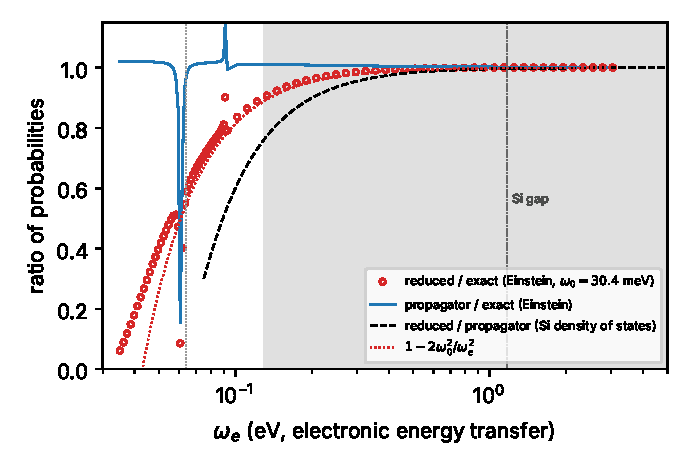
\includegraphics[width=\linewidth]{figures/ch12/limit12_4b.pdf}
\captionof{figure}{Migdal probability summed over lattice final states against the electronic energy transfer $\omega_e$, at $q = \SI{10}{keV}$ and $p = \SI{5.7}{keV}$, direction of $\vect{p}$ averaged. Circles: the reduced form over the exact second-order amplitude \cref{eq:12.4-exact} of a silicon nucleus in an isotropic harmonic well of frequency $\omega_0 = \SI{30.4}{meV}$. Solid: the unreduced propagator form \cref{eq:12.4-pm} over the same exact result; its narrow feature at $\omega_e = 2\omega_0$ is the two-phonon intermediate state, of relative weight $p^2/(2M_\kappa\omega_0) = 0.02$, which the first-order form lacks. Dotted: the leading correction $1 - 2\omega_0^2/\omega_e^2$. Dashed: reduced over propagator form with the PBE phonon spectrum of silicon (PBE band top \SI{63.7}{meV}, dotted vertical line). Gray: reduced form within \SI{10}{\percent} of the exact one, $\omega_e \ge 4.2\,\omega_0$. Dash-dotted: the silicon gap.}\label{fig:12-limit-4b}
\par}
\smallskip
The reduced form fails where $\omega_e$ approaches the phonon band, below \SI{0.20}{eV} with the silicon spectrum, where the electrons no longer see a sudden kick and the pole at $\omega_e = \omega_\nu$ turns the process into the absorption of a real phonon.
\end{limitbox}

\noindent On the truncation label \cref{lim:12.4b} sits at $n_B = 2$, with $\mathfrak{M}$ = sudden and the bound denominators $\omega_e^2 - \omega_\nu^2$, $\mathcal{K}$ = multiphonon at all orders with the lattice factor at $\vect{q}$, and $\mathcal{X}$ = random-phase with local fields. Its leading correction is one step of $n_B$, from 2 to 4: the phonon energies in the electronic denominators, of relative size $2\langle\omega_{\mathrm{ph}}^2\rangle/\omega_e^2$, as \cref{sec:8.5} counts it.

Silicon and germanium do not need the propagator. At the silicon gap of \SI{1.17}{eV} the reduced form is low by \num{2.9e-3}, at the germanium gap by about \num{3e-3}, and averaged over the silicon spectrum by \num{3e-4}. It is needed where the gap is comparable with the phonon energies: the narrow-gap and Dirac materials of \cref{chap:16}, whose gaps of tens of meV were the motivation of the phonon-mediated description, and the metals of \cref{sec:12.1-gapless}. There the region $\omega_e \lesssim 3\omega_{\mathrm{ph}}$ is not a Migdal process with a small correction but the electron--phonon response of the target.

\begin{workedexample}{The phonon-mediated term at $q = \SI{5}{keV}$}\label{we:12-five-keV}
A silicon nucleus kicked with $q = \SI{5}{keV}$ recoils with $E_R = q^2/2M_\kappa = \SI{0.478}{meV}$ and velocity $v_N = 1.91\times10^{-7}$, \SI{57}{m/s}. The momentum is reached by dark matter of $\mchi \ge q/2v_{\mathrm{max}} = \SI{0.94}{MeV}$; at \SI{1}{MeV} the largest energy transfer at this $q$, $qv_{\mathrm{max}} - q^2/2\mchi$, is \SI{0.75}{eV}, below the gap, and at \SI{2}{MeV} it is \SI{7.0}{eV}. The Debye--Waller exponent is $2W_\kappa(q) = 0.0157$. The momentum is 2.2 times $q_{\mathrm{BZ}}$, below the 2.95\,$q_{\mathrm{BZ}}$ from which \cref{sec:11.3} shows the incoherent multiphonon terms to hold and the \SI{18}{keV} from which the incoherent one-phonon term holds.

\emph{The probability.} By the sum rule of \cref{eq:12.4-harm}, the electronic spectrum is \cref{eq:12.3-soft} with the recoil energy $E_R$. At $q = 2.2\,q_{\mathrm{BZ}}$ this is the direction-averaged coherent process, within the $\vect{G} \neq \vect{G}'$ row of \cref{tab:12-nuisances}. With $Z_{\mathrm{ion}}(p)$, local fields and $\omega_e \ge \SI{1.11}{eV}$, \cref{sec:12.3} gives $6.07\times10^{-5}$ per eV of recoil energy, so $P_{\mathrm{Mig}} = 2.90\times10^{-8}$. One kick in $3.4\times10^7$ makes a pair.

\emph{The propagator.} With the PBE phonon spectrum, $\langle\omega_{\mathrm{ph}}^2\rangle^{1/2} = \SI{44.7}{meV}$. The squared bracket of \cref{eq:12.4-pmrate} times $\omega_e^4$ is 1.0029 at \SI{1.17}{eV}, the leading correction $2\langle\omega_{\mathrm{ph}}^2\rangle/\omega_e^2 = \num{2.9e-3}$, and 1.0003 averaged over the electronic spectrum, half of which lies above \SI{4.6}{eV}. The virtual phonon is far off shell, and the bound-nucleus correction is negligible.

\emph{The zero-phonon term.} With the lattice factor at $\vect{q} - \vect{p}$, \SI{96.2}{\percent} of the Migdal events leave no phonon, $P = 2.79\times10^{-8}$: the crystal takes the momentum as a whole, and all of the deposit, a few eV, is electronic. With the lattice factor at $\vect{q}$, as in \cref{eq:12.4-pmrate}, the share is \SI{98.4}{\percent}.

\emph{The phonon-emitting terms.} The rest, $1.10\times10^{-9}$, emits one phonon in \SI{96}{\percent} of the cases. Its energy follows the one-phonon spectrum of the incoherent response, $g_{\mathrm{ph},\kappa}(\omega)/\omega$, with mean $\langle\omega^{-1}\rangle^{-1} = \SI{30.4}{meV}$ and median \SI{21.7}{meV}: a phonon-emitting Migdal event gives the lattice 64 times the recoil energy. The energy comes from the dark matter, not from the recoil: kinematics bounds only the sum $\omega_e + \omega_l$, by \SI{7.0}{eV} at \SI{2}{MeV}, and a phonon costs a small part of it. Averaged over all Migdal events, the lattice receives \SI{1.20}{meV}, 2.5 times $E_R$, almost all in the rare events with a phonon.

\emph{A check.} Take a nucleus in a harmonic well of frequency \SI{30.4}{meV}, with $p = \SI{5.7}{keV}$ and $\omega_e = \SI{1.2}{eV}$. The exact amplitude \cref{eq:12.4-exact}, summed over final states, is 0.99934 times the leading form \cref{eq:12.4-lead} and 0.9980 times the propagator form \cref{eq:12.4-pm}. Its zero-phonon fraction is 0.967, against 0.984 for the lattice factor at $\vect{q}$ alone.
\end{workedexample}

The frame of the transition density, the lattice factor at small $|\vect{q} - \vect{p}|$ and the off-diagonal electronic response remain open at small momentum. The frame is the Herzberg--Teller term of \cref{sec:12.1-boost}, and at \SI{5}{keV} it is the factor 2.4 between the phonon-emitting fractions above; the electronic spectrum does not depend on it. Below $|\vect{q} - \vect{p}| \approx \SI{6.6}{keV}$ the incoherent multiphonon terms are not certified (\cref{lim:11.3a}), while the zero-phonon line, the dominant term, agrees with its diagonal, direction-averaged Bragg sum within \SI{8}{\percent}. The elements $\vect{G} \neq \vect{G}'$ of the electronic response are common to all crystal forms (\cref{app:E.18}). The frame and the lattice factor change the lattice spectrum of Migdal events, not their number, and \cref{tab:12-nuisances} carries all three.
